\documentclass[a4paper,10pt]{article}
\usepackage[utf8]{inputenc}
\usepackage[T1]{fontenc}
\usepackage[english]{babel}
\usepackage[a4paper,top=2.5cm, bottom=2.5cm, left=2.5cm, right=2.5cm]{geometry}
\usepackage{graphicx}

\title{Software Architectures\\ Assignment 1 : Design Patterns}
\author{Arnaud Rosette, Simon Picard}

\begin{document}
\maketitle%TODO : mettre une note en bas de page pour les participants pour dire qu'ils font reference au livre : design patterns book.
\section{Exercise 1 : Find Instances of Design Patterns}
\subsection{Singleton}%org.gjt.sp.jedit.syntax.ModeProvider
The org.gjt.sp.jedit.buffer.KillRing class is an instance of the singleton pattern.

\subsubsection{Purpose}
Creational pattern.
\subsubsection[Participants]{Participants\footnote[1]{The participants are those described in the book : Design Patterns: Elements of Reusable Object-Oriented Software (Gamma, Helm, Johnson, Vlissides)}}
The KillRing class is the singleton class.
\subsubsection{Class diagram}
\begin{center}
\begin{figure}[h]
  \centerline{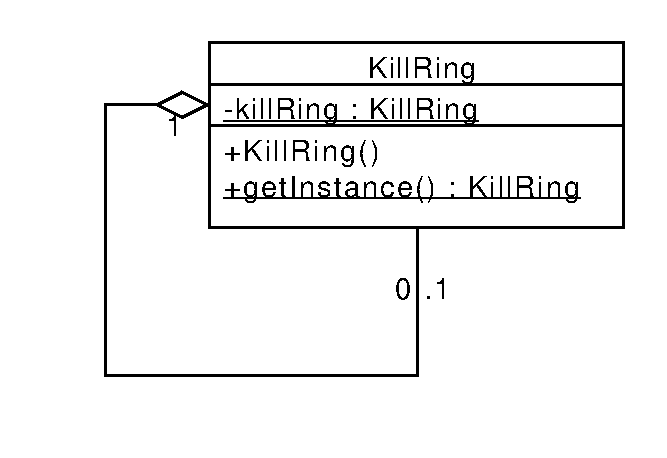
\includegraphics[width=0.5\textwidth]{singleton-killring-class-diagram.pdf}}
  \caption{KillRing class diagram}
\end{figure}
\end{center}
\subsubsection{Concrete situation description}
In this situation, the singleton pattern is used to keep track of deleted text in a single place in the application.\\
The constructor is here public. However, the common usage of the singleton pattern uses a private constructor in order to only have one instance of this class living in the system. The constructor is here made public because the plugins may want to create their own KillRing. 


\subsection{Abstract Factory}%org.gjt.sp.jedit.syntax.ModeProvider, org.gjt.sp.jedit.io.VFSManager, org.gjt.sp.jedit.gui.statusbar.StatusWidgetFactory (abstract factory) avec BufferSetWidgetFactory (concrete factory) avec Widget (abstract product) avec org.gjt.sp.jedit.gui.StatusBar (client)
The org.gjt.sp.jedit.gui.statusbar.StatusWidgetFactory class is an example of the abstract factory pattern.

\subsubsection{Purpose}
Creational pattern.
\subsubsection[Participants]{Participants\footnotemark[1]}
The participants are the classes : org.gjt.sp.jedit.gui.statusbar.StatusWidgetFactory, org.gjt.sp.jedit.gui.statusbar.BufferSetWidgetFactory, org.gjt.sp.jedit.gui.statusbar.BufferSetWidgetFactory.BufferSetWidget, org.gjt.sp.jedit.gui.statusbar.Widget and org.gjt.sp.jedit.gui.StatusBar.

\begin{itemize}
 \item \textbf{StatusWidgetFactory} : Abstract Factory
 \item \textbf{BufferSetWidgetFactory} : Concrete Factory
 \item \textbf{BufferSetWidget} : Concrete Product
 \item \textbf{Widget} : Abstract Product
 \item \textbf{StatusBar} : Client
\end{itemize}

\subsubsection{Class diagram}
\begin{center}
\begin{figure}[h]
  \centerline{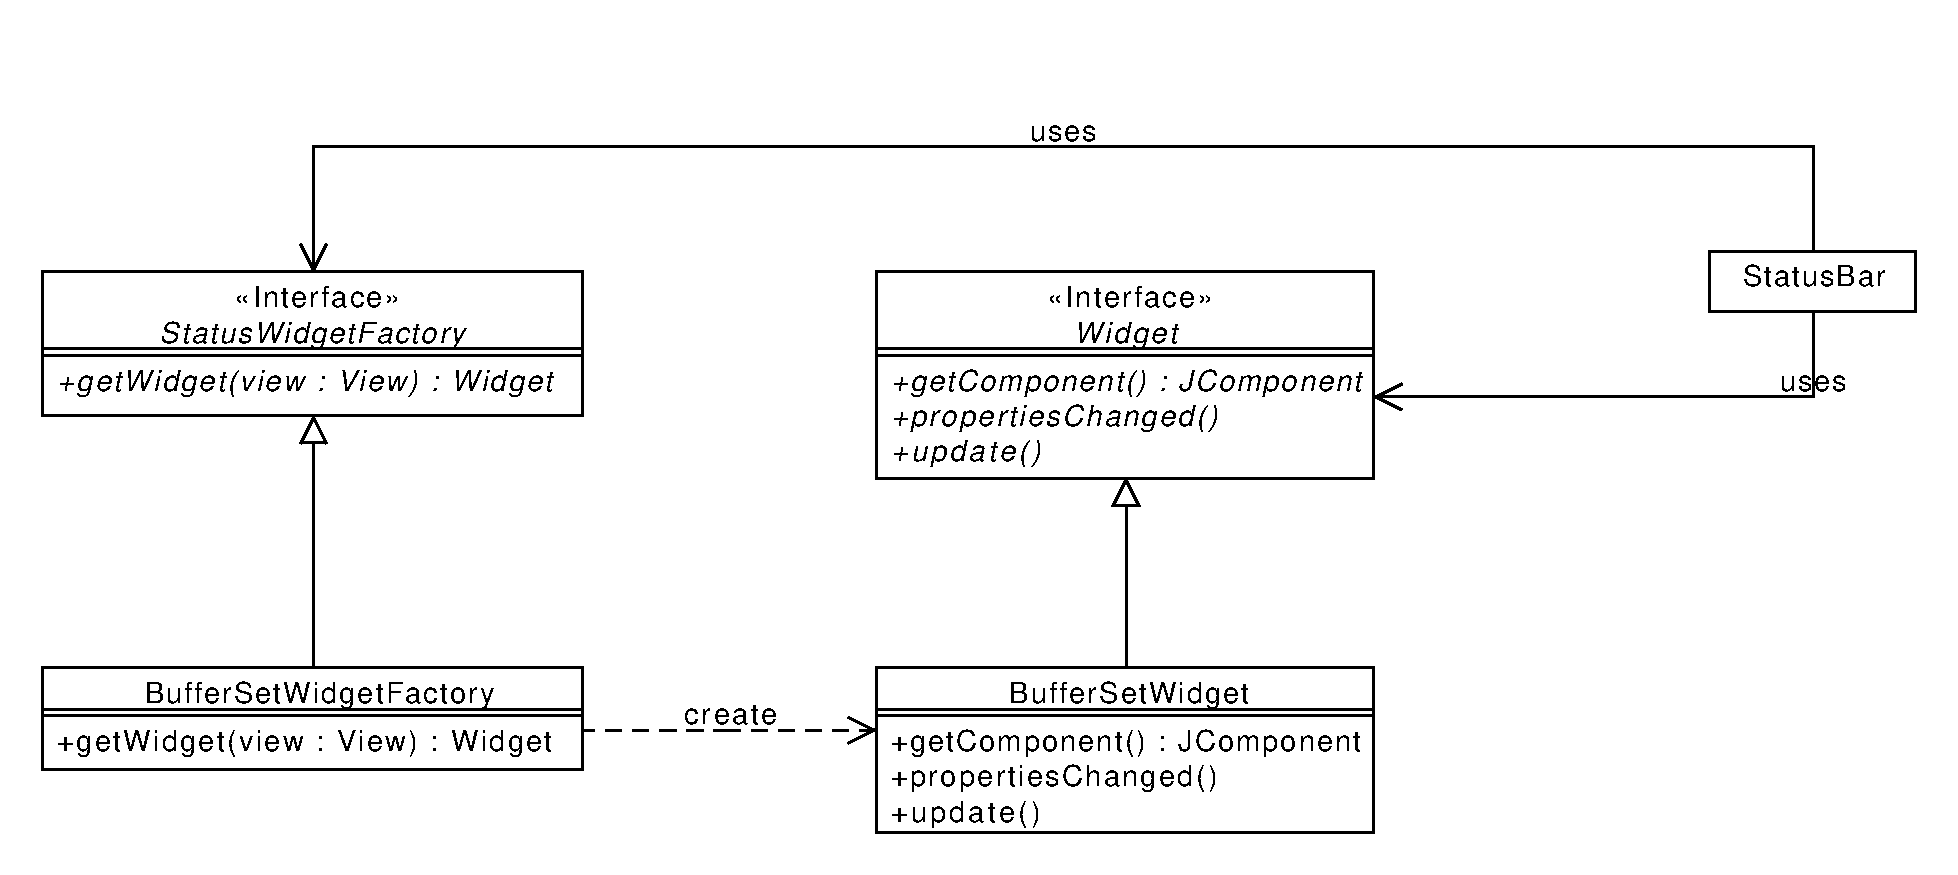
\includegraphics[width=0.9\textwidth]{abstractfactory-statuswidgetfactory-class-diagram.pdf}}
  \caption{StatusWidgetFactory class diagram}
\end{figure}
\end{center}
\subsubsection{Concrete situation description}
In this situation, the abstract factory pattern is used to let a StatusBar object creating different kind of Widget without specifying their concrete class. 

\subsection{Observer}

\subsubsection{Purpose}

\subsubsection[Participants]{Participants\footnotemark[1]}

\subsubsection{Class diagram}

\subsubsection{Concrete situation description}


\subsection{Adapter}
The org.gjt.sp.jedit.buffer.BufferAdapter class is an example of the adapter pattern.

\subsubsection{Purpose}
Structural pattern.
\subsubsection[Participants]{Participants\footnotemark[1]}
The participants are the classes : org.gjt.sp.jedit.buffer.BufferAdapter, org.gjt.sp.jedit.buffer.BufferListener, a client and a target.
\begin{itemize}
 \item \textbf{BufferAdapter} : Adapter
 \item \textbf{BufferListener} : Adaptee
\end{itemize}

\subsubsection{Class diagram}
\begin{center}
\begin{figure}[h]
  \centerline{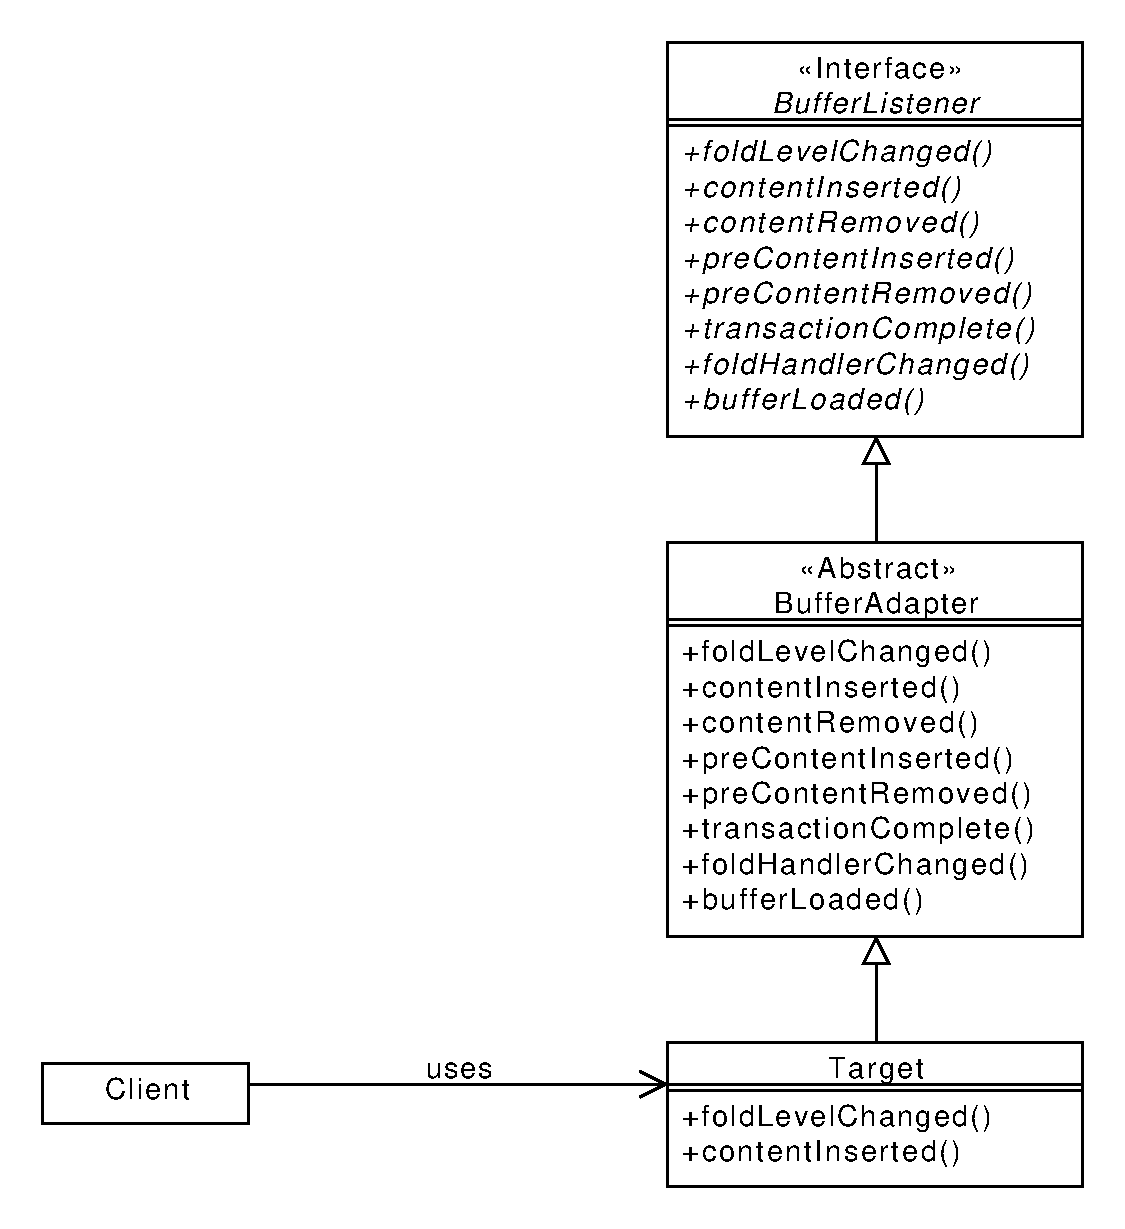
\includegraphics[width=0.5\textwidth]{adapter-bufferadapter-class-diagram.pdf}}
  \caption{BufferAdapter class diagram}
\end{figure}
\end{center}
\subsubsection{Concrete situation description}
In this situation, the BufferListener interface contains several methods but not all of them are necessary for its potential subclasses. The BufferAdapter abstract class implements all the methods of the BufferListener interface but these methods contain an empty body in order to let the next Target classes only implement the methods they need.\\
In this case, the adapter pattern is not used to let two incompatible existing classes work together but this pattern is used to let new concrete classes only implement the methods they need from this interface without implementing the methods which are not useful for these concrete classes.

\newpage
\subsection{Visitor}
The org.gjt.sp.jedit.visitors.JEditVisitor class is an example of the visitor pattern.
\subsubsection{Purpose}
Behavioral pattern.
\subsubsection[Participants]{Participants\footnotemark[1]}
The participants are the classes : org.gjt.sp.jedit.visitors.JEditVisitor, org.gjt.sp.jedit.visitors.JEditVisitorAdapter, org.gjt.sp.jedit.View.SetCursorVisitor, org.gjt.sp.jedit.visitors.SaveCaretInfoVisitor, org.gjt.sp.jedit.jEdit, org.gjt.sp.jedit.View, org.gjt.sp.jedit.EditPane and org.gjt.sp.jedit.textarea.JEditTextArea.
\begin{itemize}
 \item \textbf{JEditVisitor} : Visitor
 \item \textbf{JEditVisitorAdapter} : an Adapter that does not belong to this pattern
 \item \textbf{SetCursorVisitor} : Concrete Visitor
 \item \textbf{SaveCaretInfoVisitor} : Concrete Visitor
 \item \textbf{jEdit} : Object Structure
 \item \textbf{View} : Concrete Element and Client
 \item \textbf{EditPane} : Concrete Element
 \item \textbf{JEditTextArea} : Concrete Element
\end{itemize}

\subsubsection{Class diagram}
\begin{center}
\begin{figure}[h]
  \centerline{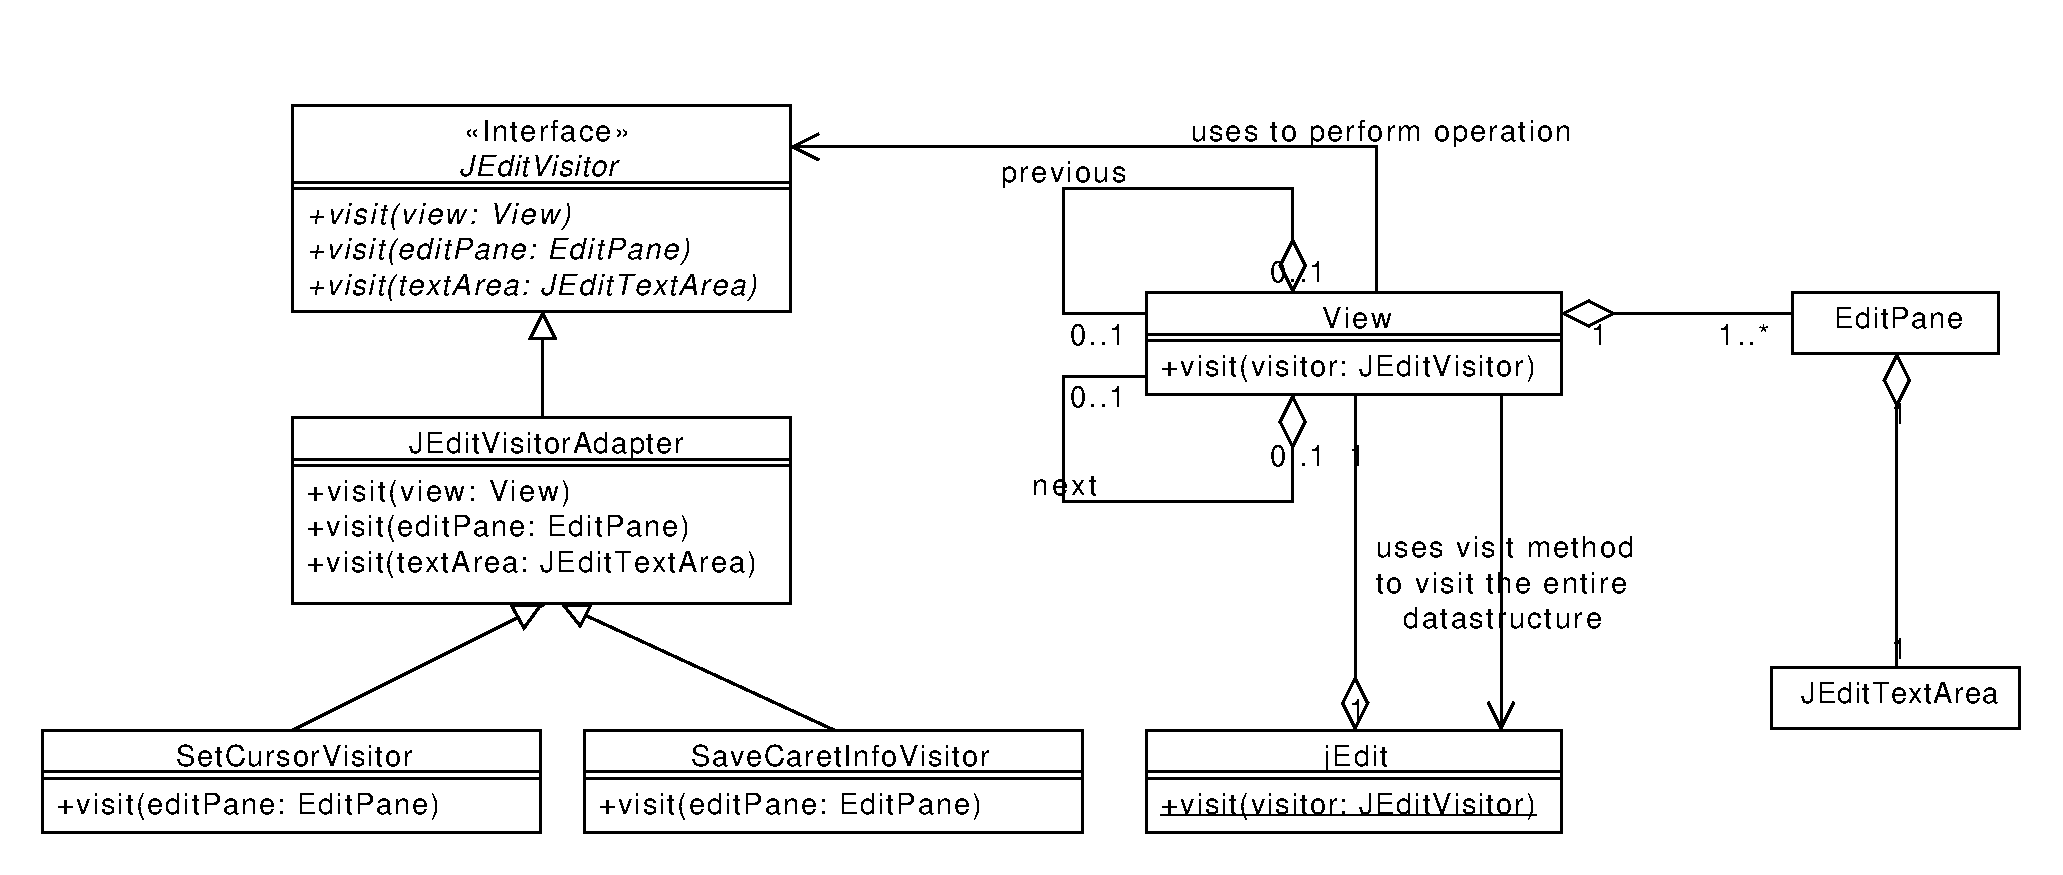
\includegraphics[width=0.9\textwidth]{visitor-jeditvisitor-class-diagram.pdf}}
  \caption{JEditVisitor class diagram}
\end{figure}
\end{center}
\subsubsection{Concrete situation description}
In this situation, the visitor design pattern is used to perform different types of action (set cursor, save caret) on a datastructure containing different types of objects. The datastructure is hold in the jEdit class (main class of the application). jEdit contains a current View and a View has references about its previous and next View. So the Views form a list structure. Further, each View may contain an EditPane and each EditPane contains a JEditTextArea.\\
A View may want to apply a specific action on the entire datastructure. In order to perform this action on the entire datastructure without depending on the concrete implementation of the elements of this datastructure, the View will use the visit method of the jEdit class by giving to it the concrete action that has to be performed, this method will visit each element of the datastructure and perform the concrete action on it.\\
The classes of the elements of the datastructure (View, EditPane, JEditTextArea) do not share a common interface. However, the theoritical version of this pattern uses a common interface between the different elements of the datastructure.


\section{Exercise 2 : Recognize Design Patterns}
The design patterns found are the command pattern (behavioural pattern) and the facade pattern (structural pattern).

\subsection{Class diagram}
\begin{center}
\begin{figure}[h]
  \centerline{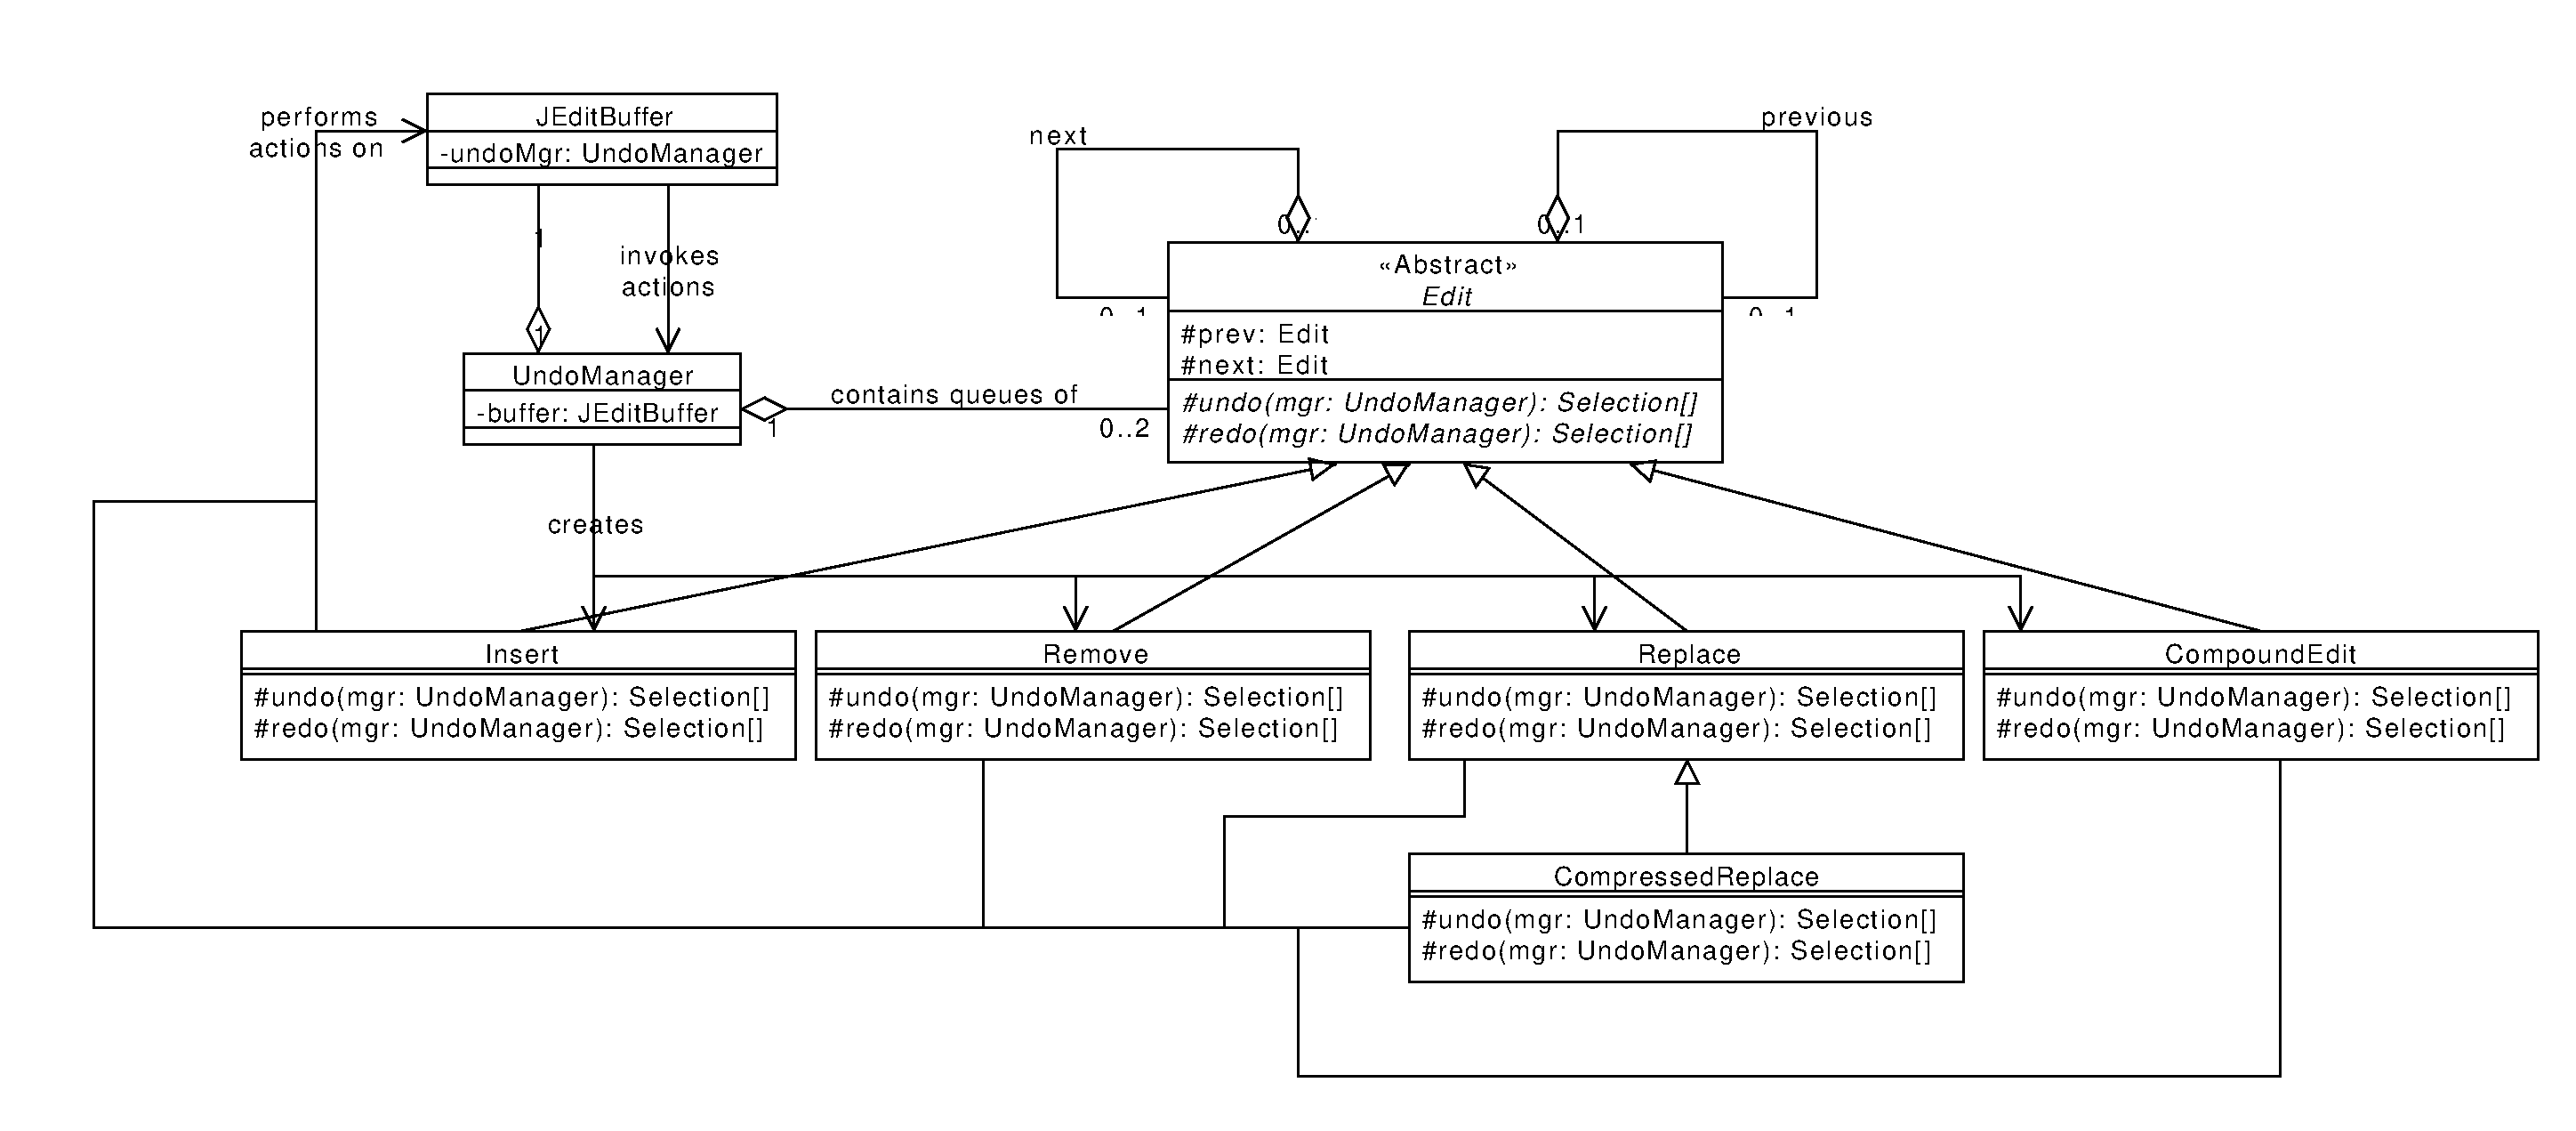
\includegraphics[width=0.9\textwidth]{undomanager-class-diagram.pdf}}
  \caption{UndoManager class diagram}
\end{figure}
\end{center}

\subsection{Command pattern}
\subsubsection{Purpose}
Behavioral pattern.
\subsubsection[Participants]{Participants\footnotemark[1]}
\begin{itemize}
 \item \textbf{Edit} : Command
 \item \textbf{Insert} : Concrete Command
 \item \textbf{Remove} : Concrete Command
 \item \textbf{Replace} : Concrete Command
 \item \textbf{CompressedReplace} : Concrete Command
 \item \textbf{CompoundEdit} : Concrete Command
 \item \textbf{UndoManager} : Client, Invoker
 \item \textbf{JEditBuffer} : Receiver
\end{itemize}

\subsubsection{Concrete situation description}
The command design pattern is used here to be able to store the actions (insert, remove, replace, ...) performed on a text (JEditBuffer). Thanks to this design pattern, the application can keep track of the actions performed during its own execution and so the application is able to undo and redo these actions. \\
The difference between this concrete case and the theoritical case is that the client and the invoker are the same object in the practical one while they are two different objects in the theory.

\subsection{Facade pattern}
\subsubsection{Purpose}
Structural pattern.
\subsubsection[Participants]{Participants\footnotemark[1]}
\begin{itemize}
 \item \textbf{Edit} : Subsystem class
 \item \textbf{Insert} : Subsystem class
 \item \textbf{Remove} : Subsystem class
 \item \textbf{Replace} : Subsystem class
 \item \textbf{CompressedReplace} : Subsystem class
 \item \textbf{CompoundEdit} : Subsystem class
 \item \textbf{UndoManager} : Facade
 \item \textbf{JEditBuffer} : Client
\end{itemize}

\subsubsection{Concrete situation description}
The facade pattern is used to hide the action classes (Insert, Remove, ...) from the rest of the application. If a class want to use these classes, it has to use the UndoManager class (facade).

\section{Exercise 3 : Coupling and Cohesion}
\subsection{Question a}
\begin{itemize}
\item A high cohesion is preferable because it means that all the function of a class are in that class for a good reason, the class has a well defined purpose.
\item A loose coupling is better because it allow the developer to modify the content of some module without jeopardize the interaction between the module and the others.
\end{itemize}
\subsection{Question b}
\subsubsection{MiscUtilities}
The cohesion type is coincidental because this class regroup all the small functions needed at several places in the projects which therefore do not have anything in common.\\
To improve the cohesion the class could be divided in several sub classes which take care of a single feature, by example, there is several functions which focus the path, they could be regrouped in one class in order to have a logical cohesion.
\subsubsection{GUIUtilities}
This class has a logical cohesion, the class handle all the function to create the GUI, they are grouped in this class because they all act in the same purpose even though they do not interact with each other.\\
The class could be sub divided to focus on single element of the GUI per classes but it will only improve the logical cohesion, in order to achieve a functional cohesion, the functions could be dispatched where they are actually useful if possible, i.e if they are not used at several places in the project.
\subsubsection{io/VFSFile.java}
This class represent an ADT, therefore the cohesion is maximal.
\subsection{Question c}
It seems that the coupling between these two classes is of the type Data because some data shared between the modules are done through parameters (e.g advanceSplashProgress).


\end{document}
